\chapter{Triangulation for Real Low-Resource Languages}
\label{chapter:reality}

\section{Four real low-resource languages}

Faced with a low-resource language pair, several questions arise when combining a direct translation model with a triangulation model:
\begin{itemize}\addtolength{\itemsep}{-0.4\baselineskip}
        \item How large should the triangulated table be?
        \item What is the best way to compute feature values in the triangulated phrase table?
        \item When combining with the direct system, do we use linear interpolation or alternative decoding paths?
        \item Is the approach of cascading a viable option?
        \item How does one penalize triangulated phrase pairs with insufficient alignment between the words in the phrase pairs?
\end{itemize}

To answer some of the above questions, we study the effectiveness of pivot-based triangulation for languages with insufficient resources, Mawukakan, Maninkakan, Malagasy and Haitian-Creole. Mawukakan and Maninkakan are two languages from the Mandekan family, spoken by almost 3.5 million people in West Africa. The Mandekan languages are a part of the Niger-Congo language family. Maninkakan and Mawukakan have little writing tradition, are written using multiple alphabets \footnote{data we have used has Latin script, obtained via LDC} and have very little resources for Machine Translation. Malagasy is the national language of Madagascar, spoken by 18 million people worldwide. Haitian-Creole is the national language of the Republic of Haiti and data used is from the Sixth Workshop on Machine translation, 2011~\cite{WMT:11}. It comprises short messages sent to the number 4636 after the devastating earthquake in January, 2010. Although nine systems participated in the workshop on Haitian-Creole, the approach of triangulation was not used. To our best knowledge, this is the first in-depth study of triangulation in a real low-resource setting and also the first for the four languages mentioned above. Mawukakan, Maninkakan and Malagasy do not have publicly available SMT systems. 

In the aftermath of the earthquake in Haiti in January, 2010, Mission 4636 set up a service where anyone in Haiti could send a message for free to a phone number 4636\footnote{\emph{http://www.mission4636.org}}. A group of volunteers translated the messages into English and helped the relief organizations provide swift help to the affected masses. Microsoft Research released a translation system to the public, for Haitian Creole, 5 days after the devastating earthquake~\cite{Lewis:11}. The fast turnaround time\footnote{\emph{To know the exact timeline, refer to http://languagelog.ldc.upenn.edu/nll/?p=2068}} and the usefulness of Machine Translation in the time of crisis inspired the featured task in the 6th Workshop on Statistical Machine Translation. Although Haitian Kreyol is a French-based Creole, approach of inducing a Haitian Kreyol to English phrase table by pivoting via French was not used.

Malagasy is an Austronesian language and the national language of Madagascar, spoken by 18 million around the world. Although it shares several words with Ma'anyan, it has influences from Arabic, French, Swahili and Bantu. Characters can have diacritics but not always. Numbers are written right-to-left like Arabic, while some words are in common with French. It follows the Latin alphabet but with 21 characters. Finally, the dataset we have is real-world news articles translated by volunteers across the world\footnote{http://www.ark.cs.cmu.edu/global-voices/} and aligned using a sentence aligner, thus, introducting some inconsistencies. 

Mawukakan\footnote{http://catalog.ldc.upenn.edu/LDC2005L01} and Maninkakan\footnote{http://catalog.ldc.upenn.edu/LDC2013L01} are two of the four languages of the Mandekan family. They have no writing tradition, are spoken by a few million people around the world and are unique in several ways. Several characters have diacritics but they can have different stress depending on the nearby words. The lengths of sentences are relatively longer when compared to English. As they have no writing tradition, there is a realistic chance they might end up as endangered languages. By using triangulation and significantly improving the output translations, we hope to preserve the existing data and encourage more monolingual and parallel data production. 

\section{Datasets}
\label{sec:datasets}


\begin{table*}
	\setlength{\tabcolsep}{4.5pt}
	%\centering
	\begin{tabular}{p{0.1\linewidth}p{0.85\linewidth}}
	\toprule
	language & src/tgt \\
	\toprule
	mawu & \emph{$\grave{a}$ $\grave{a}$ f$\acute{ɔ}$ $\acute{a}$ n$\grave{e}$ k$\grave{o}$ b$\acute{u}$l$\grave{a}$m$\acute{a}$ m$\grave{u}$s$\grave{o}$ kw$\acute{a}$$\grave{o}$ $\grave{a}$ y$\acute{a}$ w$\acute{\varepsilon}$$\acute{\varepsilon}$$\acute{o}$ l$\acute{e}$ $\acute{e}$ $\grave{a}$ m$\acute{a}$t$\acute{a}$
	$\grave{a}$} \\
	 & people say that she performs magic\\
	\midrule
	manin & \emph{$\grave{a}$l$\grave{u}$  b$\acute{a}$r$\acute{a}$ $\acute{a}$l$\acute{a}$m$\acute{a}$nd$\acute{i}$ b$\grave{e}$n $\grave{a}$ k$\grave{a}$n , k$\grave{a}$ $\grave{a}$ m$\acute{a}$s$\grave{ɔ}$r$\grave{ɔ̀}$̀  s$\acute{\varepsilon}$b$\acute{\varepsilon}$ t$\acute{\varepsilon}$ $\grave{a}$ l$\acute{a}$ 
	m$\grave{o}$r$\grave{i}$f$\grave{a}$ l$\acute{a}$} \\

	  & they fined him because his gun is not legally registered\\
	\midrule
	ht & \emph{j' aimerais avoir quelques informations svp , concernant ce numero 4636 en quoi je peux l' utiliser} \\
	&	 i would like to have information regarding the number 4636. how do i use it\\
	\midrule
	mlg & \emph{takelaa facebook ho an ` i laura sy euna efa manana mpikambana maherin  ` ny dumy arivo sahady} \\
	 & a facebook page for laura and euna already has more than five thousand members\\
	\bottomrule
	\end{tabular}
	\caption{An example for each language: mawu = Mawukakan, manin= Maninkakan, ht = Haitian Kreyol, mlg = Malagasy}
	\label{table:example_each}
\end{table*}
		


All the source sentences in Mawukakan have both French and English translations. Not all sentences in Maninkakan have both translations. The numbers for each of the datasets is mentioned in Table~\ref{table:datasettings}. The training data for Haitian Kreyol is the same as released in the Workshop. Malagasy training data also has not been changed in any manner.Both Haitian Kreyol and Malagasy have no parallel data with other languages except English. To use triangulation, we needed parallel data with atleast one more language to use as pivot. 

To enable us to reach French phrases, we have used the Bible as our source pivot text for Haitian Kreyol and Malagasy. The Bible gives us 30K sentences of text that is relatively clean. To align the Bible in source languages and French, we used hunalign~\cite{Hun:05}, a sentence aligner. No manual alignment was done. As a result of using Bible, our source pivot, pivot target and source target models are all trained on disjoint and unrelated domains for Haitian Kreyol and Malagasy. For Haitian Kreyol, we aim to improve translations for short messages using the Bible to reach french phrases present in parlimentary proceedings. For Malagasy, we aim to improve poorly aligned news articles using the Bible to reach the same french phrases. As shown in our results, we improve the translations for both over the target system. 

\subsection{Pre-processing}

    The English and French side of Mawukakan and Maninkakan parallel data sometimes have forward slashes separating equivalent english and french translations. For both, the feminine form was chosen. For instance, a sentence
    \begin{verbatim}
            he/she/it goes to school
    \end{verbatim}
            was replaced by the english sentence \\
    \begin{verbatim}
            she goes to school
    \end{verbatim}

    Text between square brackets was removed. As development, heldout and test sets are not separately released, the last 2000 sentences was used for development, heldout and test together, for both Mawukakan and Maninkakan. The top 1000 was kept aside for development, while 500 each was kept aside for heldout and test. The last 2000 sentences make up 40\% of the total data for Mawukakan and 33\% of the total data for Maninkakan. We kept aside a large percentage for development and testing to get a better idea about the difference between the various models.

    Both Haitian-Creole and Malagasy are tokenized using the French tokenizer that is part of the Moses toolkit while Mawukakan and Maninkakan are tokenized using the English tokenizer.

\subsection{Development and evaluation data}
	For Haitian Kreyol, the same development, heldout and test data has been used as the Workshop on Machine Translation. For Malagasy, the development data has been used as-is. As there is no separate heldout set, we have used the top 500 sentences of the test data as heldout, keeping aside the rest as unseen test data. 

	We used 40\% and 33\% of total data for Mawukakan and Maninkakan respectively for development, heldout and test data. A larger proportion was kept aside to make sure evaluation can be done over a range of sentences. The distribution of the evaluation data is shown in Table~\ref{table:ddtt}. The development, heldout and test sets for Haitian Kreyol have \emph{raw} and \emph{clean} versions. The raw versions are the short messages sent as-is, while the clean versions are the same messages with some words corrected or removed, e.g caf* in raw is cafe in clean version. 


\begin{table*}
	\small
	\centering
	\begin{table*}\centering
\small
\begin{tabular}{lrrr} \toprule

Paper & direct & src-pivot & pivot-tgt \\
\toprule

Utiyama '07  & 5,65,000(eparl) & 5,65,000(eparl) & 5,65,000(eparl)\\
Cohn '07 &  7,00,000(eparl) & 7,00,000(eparl) & 7,00,000(eparl) \\ 
Cohn '07 & 10,000(eparl) & 10,000(eparl) & 10,000(eparl) \\
Gispert '06 &  - & 2.18M(news) & 1.22M(news)\\
Us & 120K(SMS+OOD) & 30K(Bible) & 2M(eparl) \\
\bottomrule

\label{table:datasettings}
\end{tabular}
\caption{eparl = europarl, table shows the \#sentences in various triangulation settings}
\end{table*}


	\caption{Comparison of the low-resource scenario with Europarl}
	\label{table:datasettings}
\end{table*}


\begin{table*}
         \small
         \centering
         
\begin{tabular}{lrrr}
\toprule
Language & dev & heldout & test \\
\toprule
Mawukakan &  1000 & 500 & 500 \\
Maninkakan &  1000 & 500 & 500 \\
Haitian Kreyol & 900 & 900 & 1274 \\
Malagasy &  1133 & 500 & 633 \\
\bottomrule
\end{tabular}


         \caption{Training, development, heldout and test sets for all 4 languages}
         \label{table:ddtt}
\end{table*}



\section{Baselines}
\label{sec:baselines}
Broadly, the training data for Haitian Kreyol can be divided into 3 parts, \emph{SMS}, \emph{Out-of-domain} and \emph{Wikipedia} with 16k, 88k and 17k parallel sentences respectively. We observe, as shown in Table~\ref{table:haiti_baselines} that only using the OOD data does not take us very far. Just using the 16.6K in-domain short messages leads to a better BLEU score than not using it. Using all of the data leads to the best baseline. The \emph{bigLM} refers to an interpolated language model comprising the English side of Haitian Kreyol workshop data and the English side of Europarl. For all the other experiments, baseline-bigLM is the baseline and the same language model has been used throughout, for Haitian Kreyol. 

The baseline BLEU score for all the four languages are reported on Table~\ref{table:all_results}. Note that the baseline for Haitian-Creole outperforms the best system from the Workshop. 

\begin{table*}
	\small
	\centering
	\begin{tabular}{lllll} \toprule
System & d(cl) & d(r) & t(cl) & t(r) \\
\toprule
just-ood & 27.56 & 20.77 & 26.72 & 20.14 \\
just-sms & 32.85 & 29.15 & 32.09 & 27.56 \\
full & 33.52 & 29.76 & \emph{33.1} & 28.19 \\
full-bigLM & 33.6 & 29.83 & 33.07 & 28.91 \\ 
\bottomrule
\small
\centering
\label{table:baselines}
\end{tabular}

	\caption{Different baselines for Haitian Kreyol}
	\label{table:haiti_baselines}
\end{table*}




\section{Results}
\label{sec:results}
 The triangulated translation model alone does not achieve a comparable performance to the baseline, owing to the out-of-domain nature of the data. In our experiments, we find that Malagasy and Haitian-Creole show a linear decrease in BLEU score on the heldout set as \emph{n} is increased. Only using the triangulated translation model leads to a 14 BLEU point drop in case of Haitian-Creole, while giving a 8 point drop in case of Malagasy. Mawukakan and Maninkakan also get lower BLEU scores by only using the triangulated system. But, the optimum value of n = 100 for Mawukakan and Maninkakan. We compare the BLEU score of n = 100 and n = 1000 and saw no difference. Observing the BLEU score loss by only using the triangulated model reitaretes the importance of the direct system.  %For all the results in table~\ref{table:all_results}, the translations models are interpolated with n = 20 for Haitian-Creole and Malagasy and n = 100 for Mawukakan and Maninkakan. 
\begin{figure}[t]
                \small
                \centering
                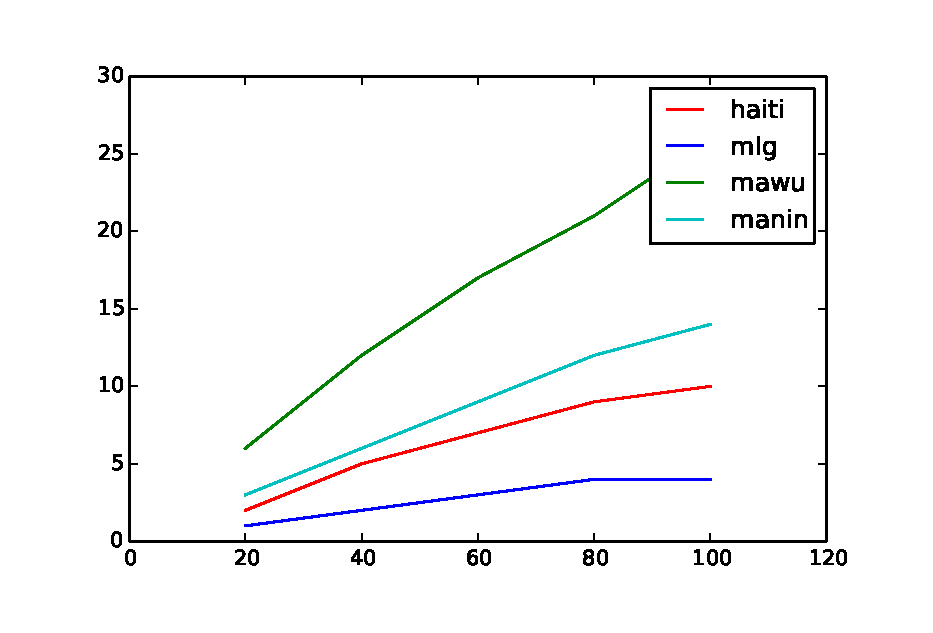
\includegraphics[scale=0.5]{files/Figures/multiplication_factors.eps}
                \caption{Linear increase in size of triangulated table as n goes from 20 to 100}
                \label{fig:multiplication_factors}

\end{figure}


Despite using a disjoint and out-of-domain Bible as source pivot and Europarl as pivot target, both Haitian-Creole and Malagasy lead to a better BLEU score on using an interpolated model comprising the direct and a top-20 triangulated model. As indicated in the example in section~\ref{sec:interpolation}, words that were mistranslated earlier get the right translations after pivoting via a large and clean fr-en phrase table.

For both Mawukakan and Maninkakan, the BLEU scores show a more significant increase of 2.2 and 1.5 BLEU points respectively for the top-n interpolation model. As the training and source pivot corpora for both comprises commonly spoken sentences that are not very long, the english side of Europarl effectively augments the limited target side of the training corpus, thus, leading to better translations after interpolation.

Intuitively, the two connectivity features should penalize the spurious and less aligned phrases, thus, reducing the noise and rewarding the just translations. But, the effect is not observed in the BLEU scores. Except in the case of Haitian-Creole where it improves by a small margin, adding the two connectivity features reduces the BLEU score. This could be owing to the fact that the source pivot data is tiny and the intersection of the alignments with the clean europarl alignments is leading to feature values that do not effectively discriminate between the good and bad. For instance, in Mawukakan and Maninkakan, 60\% and 66\% phrase pairs have a source connectivity strength of more than 0.5 while 67\% and 69\% have more than 0.5 in the backward direction. With feature values that show a more skewed distribution, the connectivity features are not helping distinguish good from bad.~\cite{Ahmed:13} found the two features useful translating Persian to Arabic via English, thus, going from a morphologically complex language to another complex language via a simpler language in the form of English.

Although Model 1 helps in the case of Malagasy and Haitian-Creole, they do not help in the other two languages. Apart from the fact that the source pivot data for both is much smaller than the Bible, the morphology of the language could have also played a role. The diacritics in Mawukakan and Maninkakan are not always used with the same stress. Sometimes, $a$ is $\acute{a}$ while sometimes it is $\grave{a}$. With Model 1's uniform initilization on a triangulated table with fewer source phrases because of the limited data, Model 1 does not always help us get better lexical scores for a given pair than the multiplied ones.

Adding the Joint and decomposed conditionals as features does well for Mawukakan and Maninkakan, leading to the best system for both. For Haitian-Creole, we replicated~\cite{Cohn:07} setting of using uniform weights for the joint probability and decomposing to find the conditions, but adding the values to the log-linear pipeline outperforms uniform interpolation of joint probabilities.


\begin{table*}
	\small
	\centering
	\begin{tabular}{lrrrr}
\toprule
Setting & Mawu & Manin & Haitian-Creole & Malagasy \\
\toprule
Baseline & 7.08 & 9.41 & 33.6 & 18.8 \\
top-n & 9.29 & 10.91 & 33.84 & 19.17 \\
top-n + Strength & 9.17  & 10.80 & 33.92 & 19.03 \\
Model 1 & 9.02 & 10.69 & 34.00 & 19.20 \\
Joint & 9.62 & 11.06 & 33.85 & - \\
\bottomrule
\end{tabular}
	\caption{Results for all languages}
	\label{table:all_results}
\end{table*}



     \begin{figure}
                \small
                \centering
                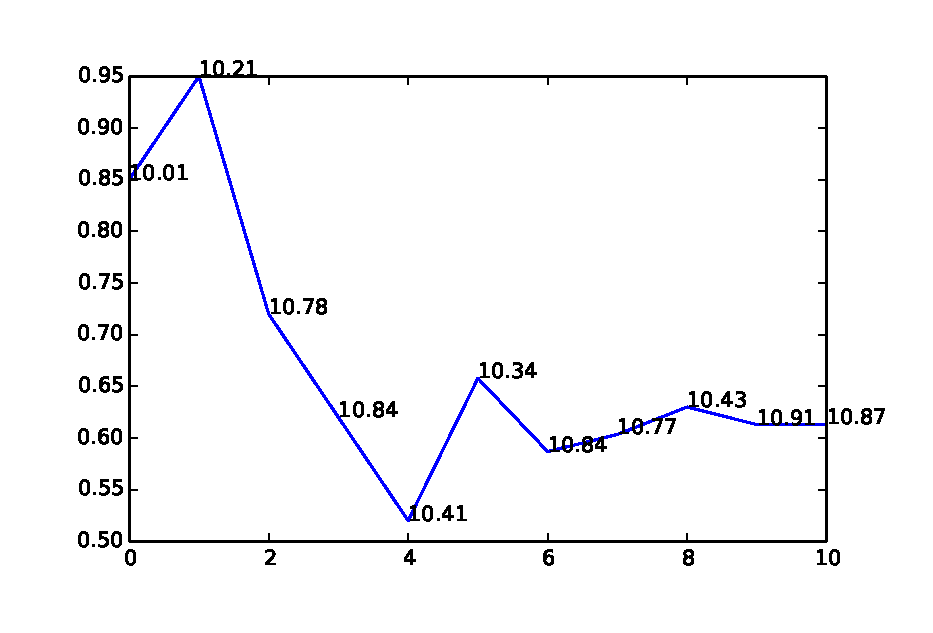
\includegraphics[width=0.45\textwidth]{files/Figures/condor_run.eps}
                \caption{Grid search over interpolation co-effs leading to a best BLEU of 10.91 using $\lambda_{d}$ = 0.612962}
                \label{fig:condor}
     \end{figure}
\begin{comment}
     \begin{figure}[ht]
     	\begin{subfigure}[b]
     		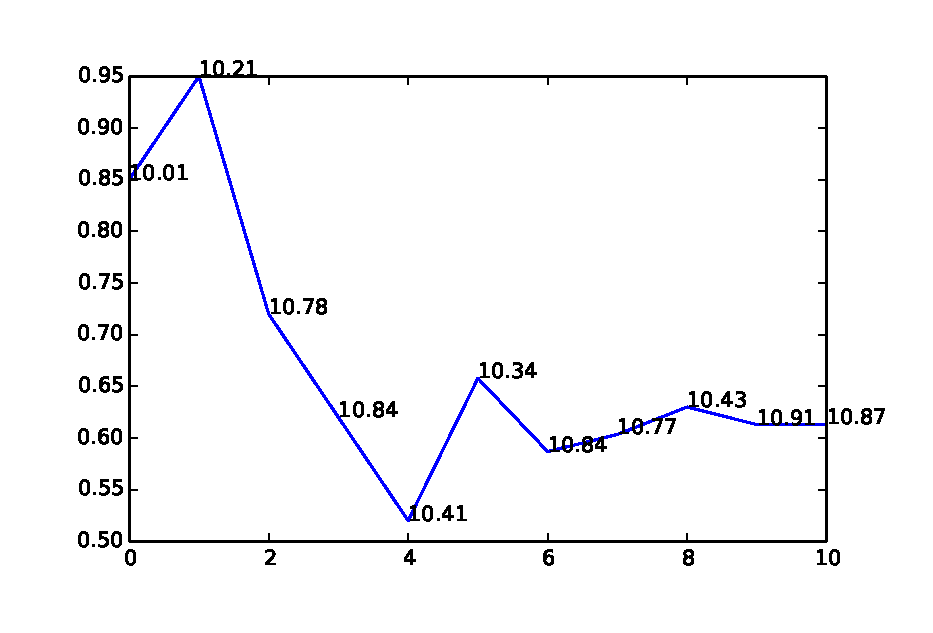
\includegraphics[scale=0.4]{files/Figures/condor_run.eps}
     	\end{subfigure} \quad
     	\begin{subfigure}[b]
     		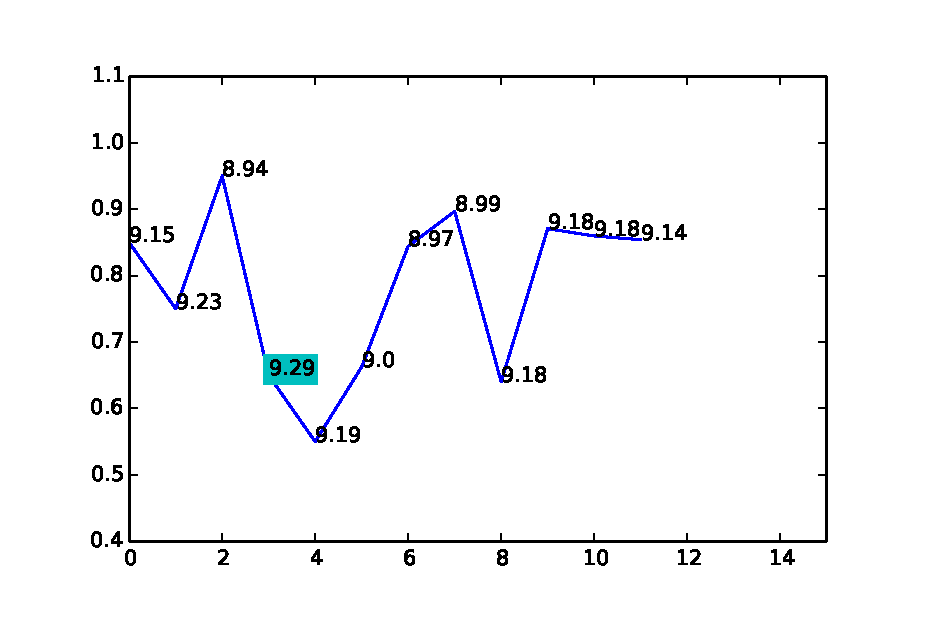
\includegraphics[scale=0.4]{files/Figures/mawut100.eps}
     	\end{subfigure} \quad
     	\small
     	\centering
     \end{figure}
\end{comment}
\section{Remarks}
\label{sec:remarks}